\section{Visualização da Solução}

O predicado print\_gold\_star/2 é utilizado para a representação de uma solução quando a estrela é constituída por 5 pontas, uma vez que é o tamanho padrão deste problema (Figura \ref{fig: print_gold_star}). Para dimensões superiores, seria necessário fazer uma função por tamanho, não sendo relevante para este trabalho.

\begin{figure}[!htb]
\hfill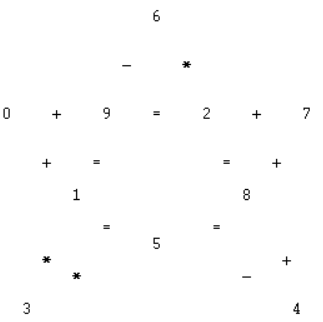
\includegraphics[width=6cm,height=6cm]{images/print_gold_star.png}\hspace*{\fill}
\caption{Exemplo do output na consola do predicado print\_gold\_star para uma solução de uma estrela de 5 pontas} \label{fig: print_gold_star}
\end{figure} 

Quando se pretende encontrar solução para uma estrela com tamanho diferente de 5, são impressas duas listas, uma com os operadores, outra com os operandos que correspondem a uma solução válida, recorrendo ao predicado print\_solution/2 (Figura \ref{fig: print_solution} ).




\begin{figure}[!htb]
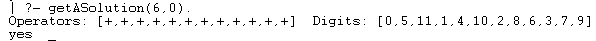
\includegraphics[width=\textwidth]{images/print_solution.png}
\caption{Exemplo do output na consola do predicado print\_solution para uma solução de uma estrela de 6 pontas} \label{fig: print_solution}
\end{figure}

A organização da lista de operadores e da lista de operandos está de acordo com a Figura \ref{fig: organizacao_estrela} .

\begin{figure}[!htb]
\hfill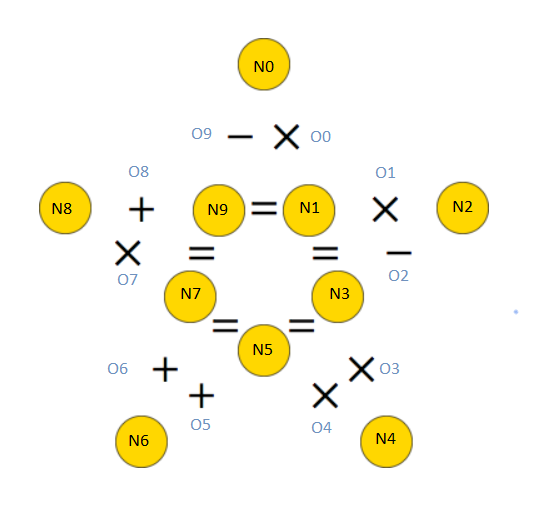
\includegraphics[width=7cm,height=7cm]{images/star_configuration.png}\hspace*{\fill}
\caption{Organização da lista de operadores e da lista de operandos para uma estrela de 5 pontas} \label{fig: organizacao_estrela}
\end{figure}

O programa contém dois predicados gerais, um para obter soluções e estas serem escritas para a consola, run/3, que recebe o predicado a ser chamado, bem como a dimensão do problema e se deve ser aplicada a restrição de check ou não, e outro para escrever para um ficheiro as soluções obtidas, save/4, que recebe o predicado a ser chamado, o nome do ficheiro em que vão ser guardadas as soluções, a dimensão do problema e se deve ou não ser aplicada a restrição check.
O predicado a ser chamado pode ser getASolution/2 que obtém uma solução para uma configuração de operaores, getConfigurationSolution/2 que obtém uma solução para cada configuração de operadores possível, getAllSolutions que obtém todas as soluções para cada configuração de operadores possível e getRandomSolution que obtém uma solução para a configuração aleatória de operadores com solução.
